\documentclass[border=6pt]{standalone}
%=======================================================================
%  ICCIT 2026 -- CAMERA-READY version, 6 pages, IEEE conference format
%  From Spikes to Sentences: A Hybrid CTC Decoder with Confidence-Gated
%  Language Model Rescoring
%  Compile: pdflatex x3, with revision_results.tex in this folder.
%=======================================================================

\usepackage{amsmath,amssymb}
\usepackage{graphicx}
\usepackage{booktabs}
\usepackage{multirow}
\usepackage{array}
\usepackage{xcolor}
\usepackage{tikz}
\usetikzlibrary{arrows.meta,positioning,calc,fit,backgrounds,shapes.geometric}
\usepackage{pgfplots}
\pgfplotsset{compat=1.17}
\usepackage{algorithm}
\usepackage{algpseudocode}
\usepackage{adjustbox}



\definecolor{ioFill}{HTML}{ECEFF4}\definecolor{ioLine}{HTML}{4C566A}
\definecolor{acFill}{HTML}{E3EEF9}\definecolor{acLine}{HTML}{3B6EA5}
\definecolor{reFill}{HTML}{E0F0EC}\definecolor{reLine}{HTML}{2E8B7F}
\definecolor{trFill}{HTML}{ECE6F5}\definecolor{trLine}{HTML}{6A4C93}
\definecolor{deFill}{HTML}{E6F0E1}\definecolor{deLine}{HTML}{4E8B3B}
\definecolor{llFill}{HTML}{FBEBDD}\definecolor{llLine}{HTML}{C1662F}
\definecolor{gaFill}{HTML}{FFF6E9}\definecolor{gaLine}{HTML}{B8860B}
\definecolor{inkLine}{HTML}{3B4252}

\tikzset{
  blk/.style={rounded corners=3pt,draw,line width=0.9pt,align=center,
              inner sep=4pt,font=\footnotesize},
  io/.style={blk,fill=ioFill,draw=ioLine},
  ac/.style={blk,fill=acFill,draw=acLine},
  re/.style={blk,fill=reFill,draw=reLine},
  tr/.style={blk,fill=trFill,draw=trLine},
  de/.style={blk,fill=deFill,draw=deLine},
  ll/.style={blk,fill=llFill,draw=llLine},
  gate/.style={diamond,aspect=1.7,draw=gaLine,fill=gaFill,line width=0.9pt,
               align=center,inner sep=1pt,font=\footnotesize},
  fl/.style={-{Stealth[length=5pt]},line width=0.9pt,draw=inkLine},
  dec/.style={-{Stealth[length=5pt]},line width=0.8pt,draw=deLine,dashed},
  tag/.style={font=\scriptsize\itshape,text=inkLine,fill=white,inner sep=1pt},
  capt/.style={font=\scriptsize,text=ioLine},
}

\newcommand{\pct}{\,\%}


\begin{document}
\setlength{\columnwidth}{3.5in}
\fontsize{10}{12}\selectfont
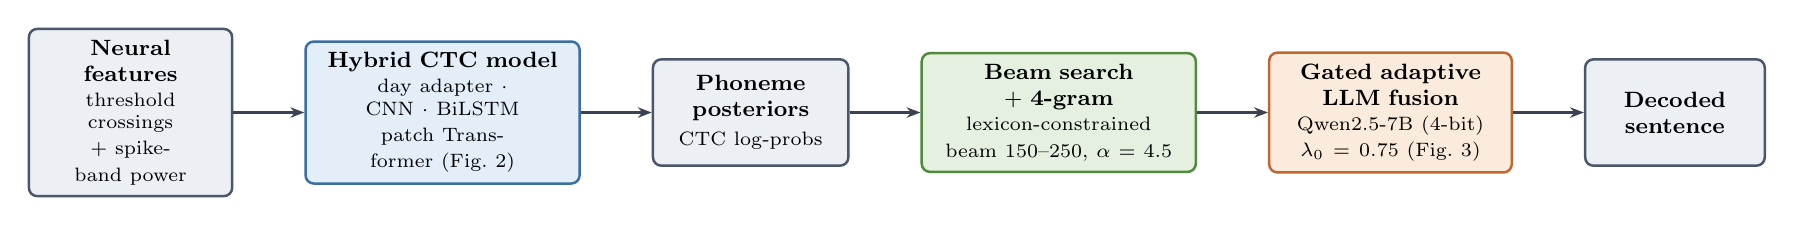
\begin{tikzpicture}[node distance=9mm]
  \node[io,minimum height=13.5mm,text width=23mm] (in)
       {\textbf{Neural}\\\textbf{features}\\[1pt]\scriptsize threshold crossings\\+ spike-band power};
  \node[ac,right=of in,minimum height=13.5mm,text width=32mm] (am)
       {\textbf{Hybrid CTC model}\\[1pt]
        \scriptsize day adapter $\cdot$ CNN $\cdot$ BiLSTM\\ patch Transformer (Fig.~2)};
  \node[io,right=of am,minimum height=13.5mm,text width=22mm] (post)
       {\textbf{Phoneme}\\\textbf{posteriors}\\[1pt]\scriptsize CTC log-probs};
  \node[de,right=of post,minimum height=13.5mm,text width=32mm] (beam)
       {\textbf{Beam search $+$ 4-gram}\\[1pt]
        \scriptsize lexicon-constrained\\ beam $150$--$250$, $\alpha=4.5$};
  \node[ll,right=of beam,minimum height=13.5mm,text width=28mm] (llm)
       {\textbf{Gated adaptive}\\\textbf{LLM fusion}\\[1pt]
        \scriptsize Qwen2.5-7B (4-bit)\\ $\lambda_0=0.75$ (Fig.~3)};
  \node[io,right=of llm,minimum height=13.5mm,text width=20mm] (out)
       {\textbf{Decoded}\\\textbf{sentence}};

  \draw[fl] (in) -- (am); \draw[fl] (am) -- (post);
  \draw[fl] (post) -- (beam); \draw[fl] (beam) -- (llm); \draw[fl] (llm) -- (out);
\end{tikzpicture}
\end{document}
